%
% This is a borrowed LaTeX template file for lecture notes for CS267,
% Applications of Parallel Computing, UCBerkeley EECS Department.
% Now being used for CMU's 10725 Fall 2012 Optimization course
% taught by Geoff Gordon and Ryan Tibshirani.  When preparing
% LaTeX notes for this class, please use this template.
%
% To familiarize yourself with this template, the body contains
% some examples of its use.  Look them over.  Then you can
% run LaTeX on this file.  After you have LaTeXed this file then
% you can look over the result either by printing it out with
% dvips or using xdvi. "pdflatex template.tex" should also work.
%

\documentclass[UTF8,oneside]{article}

% \usepackage[UTF8,scheme=plain]{ctex}
\usepackage[AutoFakeBold,AutoFakeSlant,CJKecglue]{xeCJK}  % 载入 xeCJK以支持中文,支持伪粗体,伪斜体 , 去掉CJK 文字与西文字体间的空格
\usepackage[margin=1in]{geometry}
\usepackage{amsmath,amsthm,amssymb}
\usepackage{graphicx}
\usepackage{autobreak}
\usepackage{tikz}
\usepackage{array}
\usetikzlibrary{positioning} %为了实现相对位置的设定
\usepackage{xcolor} %为了实现不同的颜色
\setCJKmainfont{宋体}                                         % 设置中文中文字体
\setCJKmonofont{宋体}                                        % 设置中文等宽字体
% \setCJKsansfont{宋体}
% \setCJKmainfont{SimSun}[BoldFont=SimHei, ItalicFont=KaiTi]
\setlength{\oddsidemargin}{0.25 in}
\setlength{\evensidemargin}{-0.25 in}
\setlength{\topmargin}{-0.6 in}
\setlength{\textwidth}{6.5 in}
\setlength{\textheight}{8.5 in}
\setlength{\headsep}{0.75 in}
\setlength{\parindent}{0 in}
\setlength{\parskip}{0.1 in}

%
% ADD PACKAGES here:
%

\usepackage{amsmath,amsfonts,graphicx}

%
% The following commands set up the lecnum (lecture number)
% counter and make various numbering schemes work relative
% to the lecture number.
%
\newcounter{lecnum}
\renewcommand{\thepage}{\thelecnum-\arabic{page}}
\renewcommand{\thesection}{\thelecnum.\arabic{section}}
\renewcommand{\theequation}{\thelecnum.\arabic{equation}}
\renewcommand{\thefigure}{\thelecnum.\arabic{figure}}
\renewcommand{\thetable}{\thelecnum.\arabic{table}}

%
% The following macro is used to generate the header.
%
\newcommand{\lecture}[4]{
   \pagestyle{myheadings}
   \thispagestyle{plain}
   \newpage
   \setcounter{lecnum}{#1}
   \setcounter{page}{1}
   \noindent
   \begin{center}
   \framebox{
      \vbox{\vspace{2mm}
    \hbox to 6.28in { {\bf Fundamentals Of Information Science
	\hfill 2022 Spring} }
       \vspace{4mm}
       \hbox to 6.28in { {\Large \hfill   #2  \hfill} }
       \vspace{2mm}
       \hbox to 6.28in { {\it 学生: #3 \hfill 时间: #4} }
      \vspace{2mm}}
   }
   \end{center}
   \markboth{Lecture #1: #2}{Lecture #1: #2}

}
%
% Convention for citations is authors' initials followed by the year.
% For example, to cite a paper by Leighton and Maggs you would type
% \cite{LM89}, and to cite a paper by Strassen you would type \cite{S69}.
% (To avoid bibliography problems, for now we redefine the \cite command.)
% Also commands that create a suitable format for the reference list.
\renewcommand{\cite}[1]{[#1]}
\def\beginrefs{\begin{list}%
        {[\arabic{equation}]}{\usecounter{equation}
         \setlength{\leftmargin}{2.0truecm}\setlength{\labelsep}{0.4truecm}%
         \setlength{\labelwidth}{1.6truecm}}}
\def\endrefs{\end{list}}
\def\bibentry#1{\item[\hbox{[#1]}]}

%Use this command for a figure; it puts a figure in wherever you want it.
%usage: \fig{NUMBER}{SPACE-IN-INCHES}{CAPTION}
\newcommand{\fig}[3]{
			\vspace{#2}
			\begin{center}
			Figure \thelecnum.#1:~#3
			\end{center}
	}
% Use these for theorems, lemmas, proofs, etc.
\usepackage{amsthm}
\newtheorem*{Solution}{Solution}
\newtheorem{theorem}{Theorem}[lecnum]
\newtheorem{lemma}[theorem]{Lemma}

\newtheorem{proposition}[theorem]{Proposition}
\newtheorem{claim}[theorem]{Claim}
\newtheorem{corollary}[theorem]{Corollary}
\newtheorem{definition}[theorem]{Definition}
% \newenvironment{proof}{{\bf Proof:}}{\hfill\rule{2mm}{2mm}}

% **** IF YOU WANT TO DEFINE ADDITIONAL MACROS FOR YOURSELF, PUT THEM HERE:

\newcommand\E{\mathbb{E}}

\begin{document}
%FILL IN THE RIGHT INFO.
%\lecture{**LECTURE-NUMBER**}{**DATE**}{**LECTURER**}{**SCRIBE**}
\lecture{1}{Homework9}{华园(202000120027))}{2022.3.23}
%\footnotetext{These notes are partially based on those of Nigel Mansell.}

% **** YOUR NOTES GO HERE:

% Some general latex examples and examples making use of the
% macros follow.
%**** IN GENERAL, BE BRIEF. LONG SCRIBE NOTES, NO MATTER HOW WELL WRITTEN,
%**** ARE NEVER READ BY ANYBODY.

\section*{Problem 1.} % Don't be this informal in your notes!
Ciphertext expansion vs. security\\
Let $\mathcal{E}=(E, D)$ be an encryption scheme messages and ciphertexts are bit strings.\\
(a) Suppose that for all keys and all messages $m$, the encryption of $m$ is the exact same length as $m$. Show that $(E, D)$ cannót be semantically secure under a chosen plaintext attack.\\
(b) Suppose that for all keys and all messages $m$, the encryption of $m$ is exactly $\ell$ bits longer than the length of $m$. Show an attacker that can win the CPA security game using $\approx 2^{\ell} / 2$ queries and advantage $\approx 1 / 2$. You may assume the message space contains more than $\approx 2^{\ell} / 2$ messages.

\begin{Solution}
\end{Solution}
(a)
\begin{center}
  \begin{tikzpicture}
\draw  [black](-1,2)--(-1,-2);
\draw  [black](-1,2)--(-3,2);
\draw  [black](-3,2)--(-3,-2);
\draw  [black](-3,-2)--(-1,-2);

\draw  [black](1,2)--(1,-2);
\draw  [black](1,2)--(3,2);
\draw  [black](3,2)--(3,-2);
\draw  [black](3,-2)--(1,-2);

\draw  [black,->](1,1.5)--node[below=-14pt,fill=white]{$m_0,m_0$}(-1,1.5);
\draw  [black,->](-1,0.5)--node[below=-17.5pt,fill=white]{$E(k,m_0)$}(1,0.5);
\draw  [black,->](1,-0.5)--node[below=-14pt,fill=white]{$m_0,m_1$}(-1,-0.5);
\draw  [black,->](-1,-1.5)--node[below=-17.5pt,fill=white]{$E(k,m_b)$}(1,-1.5);


\draw  [black,->](-2,2.5)--node[below=-17pt,fill=white]{$b$}(-2,2);
\draw  [black,->](2,-2)--node[below=7pt,fill=white]{$b'$}(2,-2.5);

\filldraw [black] (-2,1) circle (0pt)--node[fill=white]{$chal$}(-2,1);
\filldraw [black] (2,1) circle (0pt)--node[fill=white]{$Adv$}(2,1);
\filldraw [black] (-2,-1) circle (0pt)--node[fill=white]{$k\leftarrow K$}(-2,-1);
  \end{tikzpicture}
\end{center}
由于CPA中多次询问用同一个密钥加密按照,所以上图的思路进行攻击,首先第一次发送两个相同的明文$m_0$,无论b等于0还是1,都会对$m_0$进行加密,因此我们可以获取到$m_0$加密后的密文。第二次攻击我们发送两条不同的明文$m_0$和$m_1$,系统会随机选取一个进行加密,然后我们收到密文,通过对比第一次获得的明文,我们就可以判断出加密的是$m_0$还是$m_1$,从而可以判断出b的数值,即:$$Adv_{ss}=|Pr(W_0)-Pr(W_1)|=1$$
这个结果是不可忽略的,因此不是语意安全的。\\
(b)问题分析:密文长度长于明文长度,即密文包括两部分,其中一部分是用密钥加密,另一部分是l位的随机数,攻击者获得CPA游戏胜利的条件是:能够根据密文区分出是$m_0$加密的还是$m_1$加密的。现在我们知道:攻击者具有的能力是具有$\frac{1}{2}$的概率识别出b的数值,同时有$2^{l-1}$次查询机会,现在我们需要证明的是,在剩下的不能识别的$\frac{1}{2}$中可以通过查询message space来获取明文。\\
证明:\\message space空间包含多于$2^{l-1}$的消息,因为在CPA游戏中,使用的key是一样的,因此密文的不同之处就在于随机数的不同,则在剩余的$\frac{1}{2}$中最多需要查询次数$$\frac{1}{2}2^l=2^l/2$$
这样就一定可以从中找到相对应的明文和密文对,从而可以判断出b的值,因此结论得证。
\section*{Problem 2.}
Understand public-key encryption\\
Given two random primers $(p, q)=(31,43)$, you are asked to construct an RSA encryption based on the two primes $(p, q)$ (although the primes are two small to guarantee security).\\
(a) Construct a pair of public key and secret key.\\
(b) Demonstrate the process of encrypting a message $m=100$ with a random number $x=13$ using the generated key pair, and then decrypt the resulting ciphertext.
\begin{Solution}
\end{Solution}
(a)由题目条件可知,p=31,q=43,则有$$N=qp=1333$$
则我们可以获得非p的整数倍和非q的整数倍的数字的个数为:$$\varphi(N)=(p-1)(q-1)=N-p-q+1=1260$$
则需要寻找一对整数e.d使得e·d mod $\varphi(N)$=1,经过计算获得e=13,d=97.因此我们可以获得公钥为(1333,13),私钥为(1333,97)\\
(b)我们假设加密的方式为(E,D),K为(E,D)的密钥空间,假设H()为从$Z_N$到K的映射。则整个通信过程:
针对发送方:\\
(1)生成公钥(1333,13)和密钥(1333,97)\\
(2)对随机数x进行RSA处理获得y:$$y=x^{13} mod1333=864$$
(3)将随机数映射到K空间获得,$$k=H(x)=H(13)$$
(3)利用k=H(13)对m进行加密,获得:$$E(k,m)=E(H(13),100)$$
(4)发送方输出(y,E(k,m)),即输出(864,E(H(13),100))$$ $$
针对接收方:\\
(1)接收到发送方消息之后,利用私钥97对y进行解密获得随机数x:$$x=y^{97} mod 1333=13$$
(2)之后利用映射关系获得密钥:$$k=H(x)=H(13)$$
(3)获得密钥之后,对获得的密文进行解密:$$m=D(k,E(k,m))=D(H(13),E(H(13),100))=100$$

% **** THIS ENDS THE EXAMPLES. DON'T DELETE THE FOLLOWING LINE:

\end{document}





